\section{PToPSwitchArbiterVcs Class Reference}
\label{classPToPSwitchArbiterVcs}\index{PToPSwitchArbiterVcs@{PToPSwitchArbiterVcs}}
{\tt \#include $<$ptopSwaVcs.h$>$}

Collaboration diagram for PToPSwitchArbiterVcs:\nopagebreak
\begin{figure}[H]
\begin{center}
\leavevmode
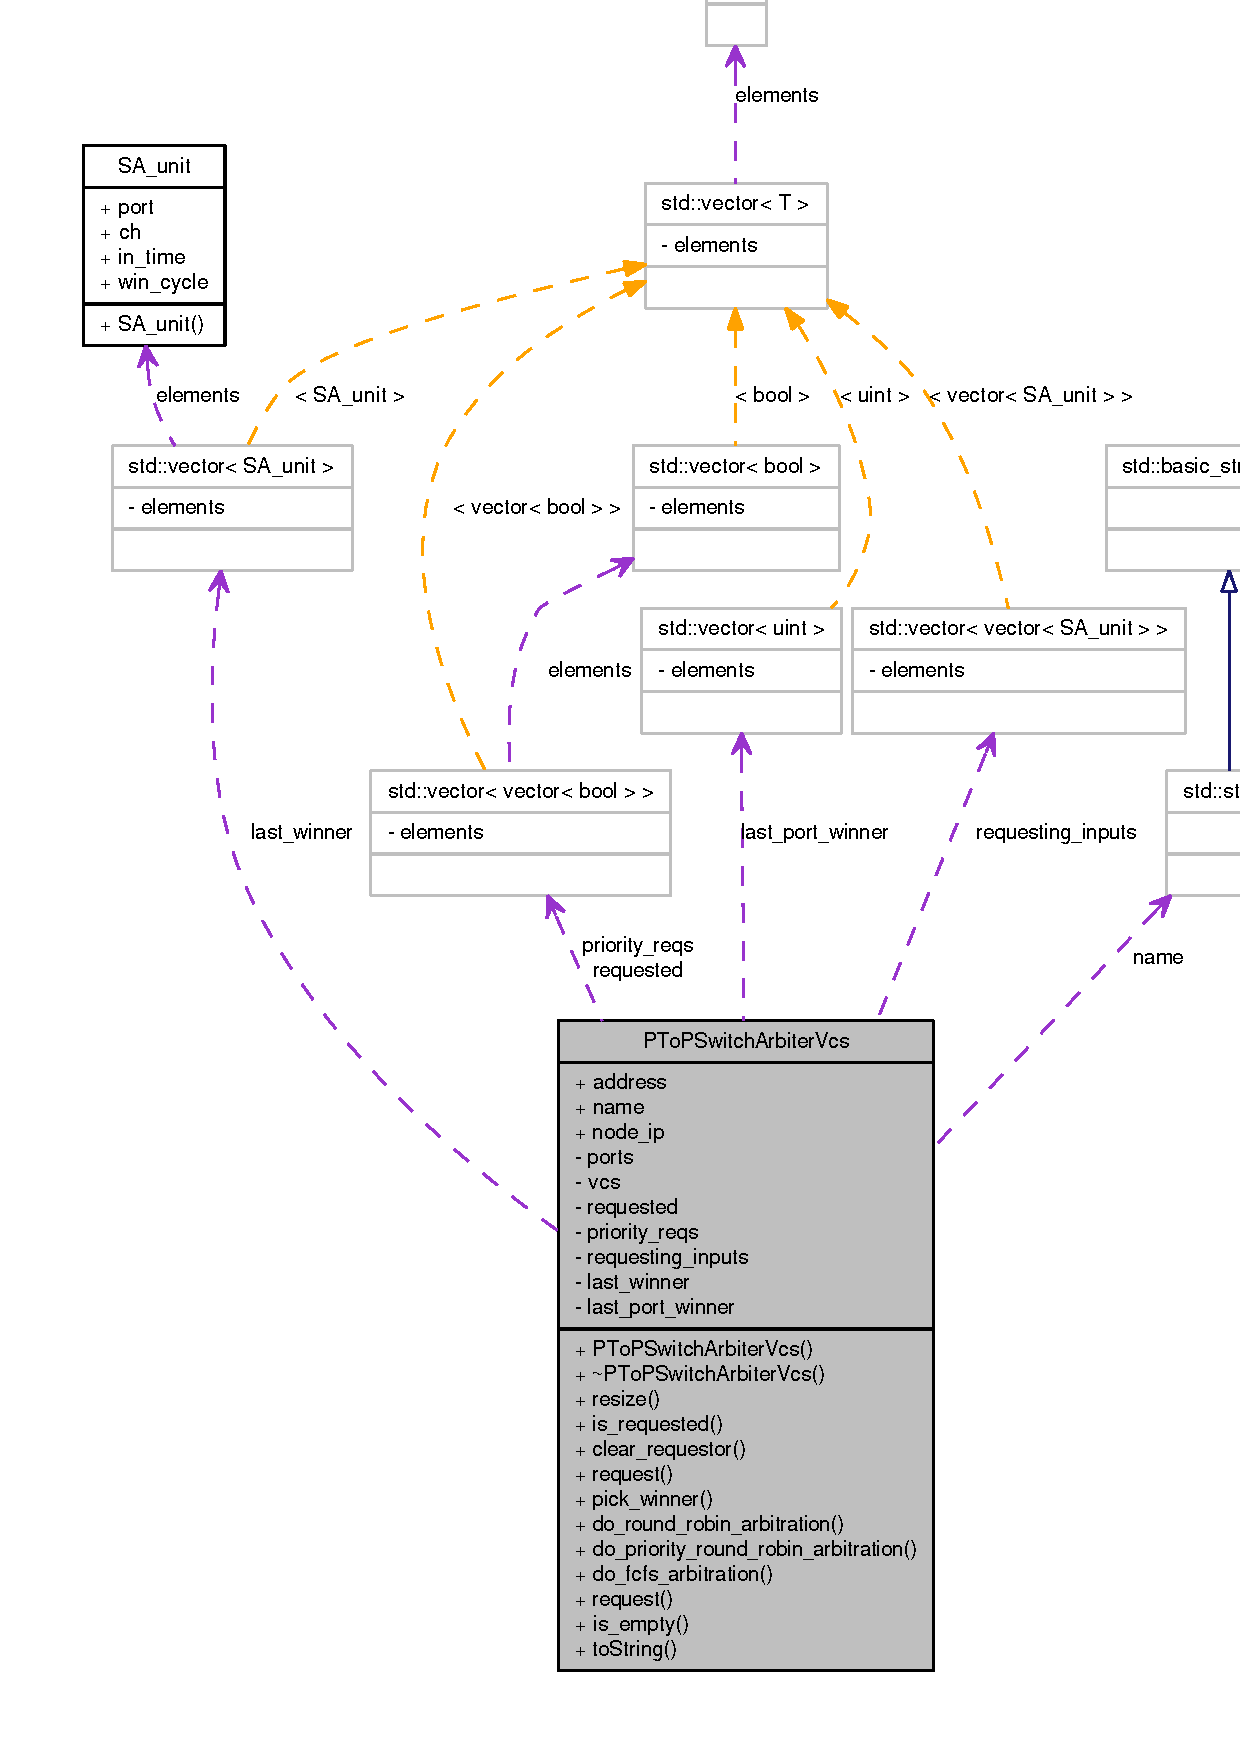
\includegraphics[width=400pt]{classPToPSwitchArbiterVcs__coll__graph}
\end{center}
\end{figure}
\subsection*{Public Member Functions}
\begin{CompactItemize}
\item 
{\bf PToPSwitchArbiterVcs} ()
\item 
{\bf $\sim$PToPSwitchArbiterVcs} ()
\item 
void {\bf resize} ({\bf uint} p, {\bf uint} v)
\item 
bool {\bf is\_\-requested} ({\bf uint} outp, {\bf uint} inp, {\bf uint} ovc)
\item 
void {\bf clear\_\-requestor} ({\bf uint} outp, {\bf uint} inp, {\bf uint} ovc)
\item 
void {\bf request} ({\bf uint} p, {\bf uint} op, {\bf uint} inp, {\bf uint} iv)
\item 
{\bf SA\_\-unit} {\bf pick\_\-winner} ({\bf uint} p)
\item 
{\bf SA\_\-unit} {\bf do\_\-round\_\-robin\_\-arbitration} ({\bf uint} p)
\item 
{\bf SA\_\-unit} {\bf do\_\-priority\_\-round\_\-robin\_\-arbitration} ({\bf uint} p)
\item 
{\bf SA\_\-unit} {\bf do\_\-fcfs\_\-arbitration} ({\bf uint} p)
\item 
void {\bf request} ({\bf uint} oport, {\bf uint} inport, {\bf message\_\-class} m)
\item 
bool {\bf is\_\-empty} ()
\item 
string {\bf toString} () const 
\end{CompactItemize}
\subsection*{Public Attributes}
\begin{CompactItemize}
\item 
{\bf uint} {\bf address}
\item 
string {\bf name}
\item 
{\bf uint} {\bf node\_\-ip}
\end{CompactItemize}
\subsection*{Private Attributes}
\begin{CompactItemize}
\item 
{\bf uint} {\bf ports}
\item 
{\bf uint} {\bf vcs}
\item 
vector$<$ vector$<$ bool $>$ $>$ {\bf requested}
\item 
vector$<$ vector$<$ bool $>$ $>$ {\bf priority\_\-reqs}
\item 
vector$<$ vector$<$ {\bf SA\_\-unit} $>$ $>$ {\bf requesting\_\-inputs}
\item 
vector$<$ {\bf SA\_\-unit} $>$ {\bf last\_\-winner}
\item 
vector$<$ {\bf uint} $>$ {\bf last\_\-port\_\-winner}
\end{CompactItemize}


\subsection{Detailed Description}


Definition at line 30 of file ptopSwaVcs.h.

\subsection{Constructor \& Destructor Documentation}
\index{PToPSwitchArbiterVcs@{PToPSwitchArbiterVcs}!PToPSwitchArbiterVcs@{PToPSwitchArbiterVcs}}
\index{PToPSwitchArbiterVcs@{PToPSwitchArbiterVcs}!PToPSwitchArbiterVcs@{PToPSwitchArbiterVcs}}
\subsubsection[{PToPSwitchArbiterVcs}]{\setlength{\rightskip}{0pt plus 5cm}PToPSwitchArbiterVcs::PToPSwitchArbiterVcs ()}\label{classPToPSwitchArbiterVcs_5530a6bc568a9e855ece521371534231}




Definition at line 24 of file ptopSwaVcs.cc.

References name.\index{PToPSwitchArbiterVcs@{PToPSwitchArbiterVcs}!$\sim$PToPSwitchArbiterVcs@{$\sim$PToPSwitchArbiterVcs}}
\index{$\sim$PToPSwitchArbiterVcs@{$\sim$PToPSwitchArbiterVcs}!PToPSwitchArbiterVcs@{PToPSwitchArbiterVcs}}
\subsubsection[{$\sim$PToPSwitchArbiterVcs}]{\setlength{\rightskip}{0pt plus 5cm}PToPSwitchArbiterVcs::$\sim$PToPSwitchArbiterVcs ()}\label{classPToPSwitchArbiterVcs_a4dfd3e859f494b925f1089d9e201c0b}




Definition at line 29 of file ptopSwaVcs.cc.

\subsection{Member Function Documentation}
\index{PToPSwitchArbiterVcs@{PToPSwitchArbiterVcs}!clear\_\-requestor@{clear\_\-requestor}}
\index{clear\_\-requestor@{clear\_\-requestor}!PToPSwitchArbiterVcs@{PToPSwitchArbiterVcs}}
\subsubsection[{clear\_\-requestor}]{\setlength{\rightskip}{0pt plus 5cm}void PToPSwitchArbiterVcs::clear\_\-requestor ({\bf uint} {\em outp}, \/  {\bf uint} {\em inp}, \/  {\bf uint} {\em ovc})}\label{classPToPSwitchArbiterVcs_78a137f4c943b0e2fe41ec07cf744d8c}




Definition at line 136 of file ptopSwaVcs.cc.

References requested, and vcs.

Referenced by GenericRouterVcs::do\_\-switch\_\-allocation(), and GenericRouterVcs::do\_\-switch\_\-traversal().

Here is the caller graph for this function:\nopagebreak
\begin{figure}[H]
\begin{center}
\leavevmode
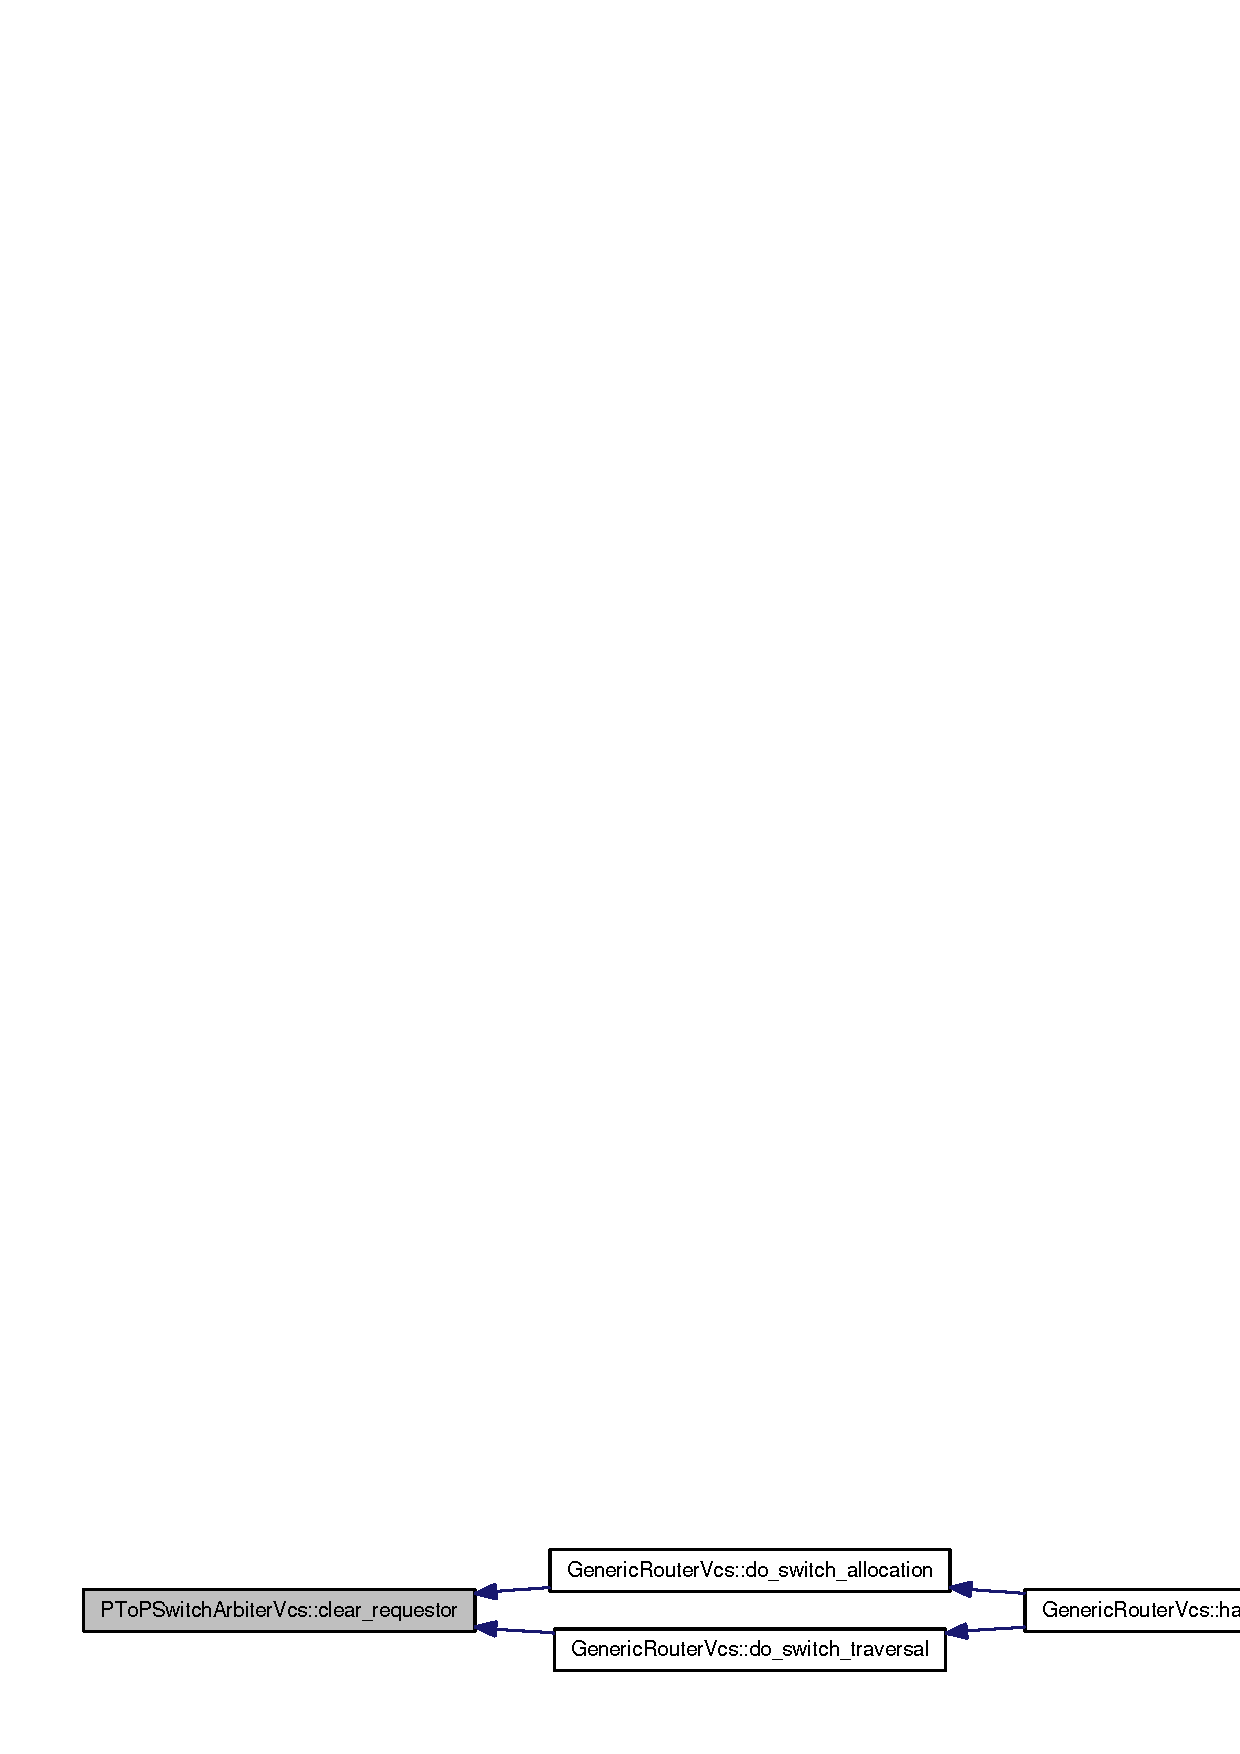
\includegraphics[width=420pt]{classPToPSwitchArbiterVcs_78a137f4c943b0e2fe41ec07cf744d8c_icgraph}
\end{center}
\end{figure}
\index{PToPSwitchArbiterVcs@{PToPSwitchArbiterVcs}!do\_\-fcfs\_\-arbitration@{do\_\-fcfs\_\-arbitration}}
\index{do\_\-fcfs\_\-arbitration@{do\_\-fcfs\_\-arbitration}!PToPSwitchArbiterVcs@{PToPSwitchArbiterVcs}}
\subsubsection[{do\_\-fcfs\_\-arbitration}]{\setlength{\rightskip}{0pt plus 5cm}{\bf SA\_\-unit} PToPSwitchArbiterVcs::do\_\-fcfs\_\-arbitration ({\bf uint} {\em p})}\label{classPToPSwitchArbiterVcs_1c0ac30090af685d204d4b2ea12ec522}


\index{PToPSwitchArbiterVcs@{PToPSwitchArbiterVcs}!do\_\-priority\_\-round\_\-robin\_\-arbitration@{do\_\-priority\_\-round\_\-robin\_\-arbitration}}
\index{do\_\-priority\_\-round\_\-robin\_\-arbitration@{do\_\-priority\_\-round\_\-robin\_\-arbitration}!PToPSwitchArbiterVcs@{PToPSwitchArbiterVcs}}
\subsubsection[{do\_\-priority\_\-round\_\-robin\_\-arbitration}]{\setlength{\rightskip}{0pt plus 5cm}{\bf SA\_\-unit} PToPSwitchArbiterVcs::do\_\-priority\_\-round\_\-robin\_\-arbitration ({\bf uint} {\em p})}\label{classPToPSwitchArbiterVcs_f93133346164b48460122959cb08b763}


\index{PToPSwitchArbiterVcs@{PToPSwitchArbiterVcs}!do\_\-round\_\-robin\_\-arbitration@{do\_\-round\_\-robin\_\-arbitration}}
\index{do\_\-round\_\-robin\_\-arbitration@{do\_\-round\_\-robin\_\-arbitration}!PToPSwitchArbiterVcs@{PToPSwitchArbiterVcs}}
\subsubsection[{do\_\-round\_\-robin\_\-arbitration}]{\setlength{\rightskip}{0pt plus 5cm}{\bf SA\_\-unit} PToPSwitchArbiterVcs::do\_\-round\_\-robin\_\-arbitration ({\bf uint} {\em p})}\label{classPToPSwitchArbiterVcs_e8adb19a43c5674bae5f4cab64b58a14}




Definition at line 90 of file ptopSwaVcs.cc.

References \_\-DBG\_\-NOARG, last\_\-port\_\-winner, last\_\-winner, Simulator::Now(), ports, requested, requesting\_\-inputs, and vcs.

Referenced by pick\_\-winner().

Here is the caller graph for this function:\nopagebreak
\begin{figure}[H]
\begin{center}
\leavevmode
\includegraphics[width=420pt]{classPToPSwitchArbiterVcs_e8adb19a43c5674bae5f4cab64b58a14_icgraph}
\end{center}
\end{figure}
\index{PToPSwitchArbiterVcs@{PToPSwitchArbiterVcs}!is\_\-empty@{is\_\-empty}}
\index{is\_\-empty@{is\_\-empty}!PToPSwitchArbiterVcs@{PToPSwitchArbiterVcs}}
\subsubsection[{is\_\-empty}]{\setlength{\rightskip}{0pt plus 5cm}bool PToPSwitchArbiterVcs::is\_\-empty (void)}\label{classPToPSwitchArbiterVcs_a346b5f33fbb252e2ec942caa7243922}




Definition at line 144 of file ptopSwaVcs.cc.

References ports, requested, and vcs.

Referenced by GenericRouterVcs::do\_\-switch\_\-allocation().

Here is the caller graph for this function:\nopagebreak
\begin{figure}[H]
\begin{center}
\leavevmode
\includegraphics[width=420pt]{classPToPSwitchArbiterVcs_a346b5f33fbb252e2ec942caa7243922_icgraph}
\end{center}
\end{figure}
\index{PToPSwitchArbiterVcs@{PToPSwitchArbiterVcs}!is\_\-requested@{is\_\-requested}}
\index{is\_\-requested@{is\_\-requested}!PToPSwitchArbiterVcs@{PToPSwitchArbiterVcs}}
\subsubsection[{is\_\-requested}]{\setlength{\rightskip}{0pt plus 5cm}bool PToPSwitchArbiterVcs::is\_\-requested ({\bf uint} {\em outp}, \/  {\bf uint} {\em inp}, \/  {\bf uint} {\em ovc})}\label{classPToPSwitchArbiterVcs_b260fc3fbec7be3f4c5cce7a73d96bca}




Definition at line 63 of file ptopSwaVcs.cc.

References ports, requested, and vcs.\index{PToPSwitchArbiterVcs@{PToPSwitchArbiterVcs}!pick\_\-winner@{pick\_\-winner}}
\index{pick\_\-winner@{pick\_\-winner}!PToPSwitchArbiterVcs@{PToPSwitchArbiterVcs}}
\subsubsection[{pick\_\-winner}]{\setlength{\rightskip}{0pt plus 5cm}{\bf SA\_\-unit} PToPSwitchArbiterVcs::pick\_\-winner ({\bf uint} {\em p})}\label{classPToPSwitchArbiterVcs_39274b4ccaad44c9217f150a30bba0e7}




Definition at line 84 of file ptopSwaVcs.cc.

References do\_\-round\_\-robin\_\-arbitration().

Referenced by GenericRouterVcs::do\_\-switch\_\-allocation().

Here is the caller graph for this function:\nopagebreak
\begin{figure}[H]
\begin{center}
\leavevmode
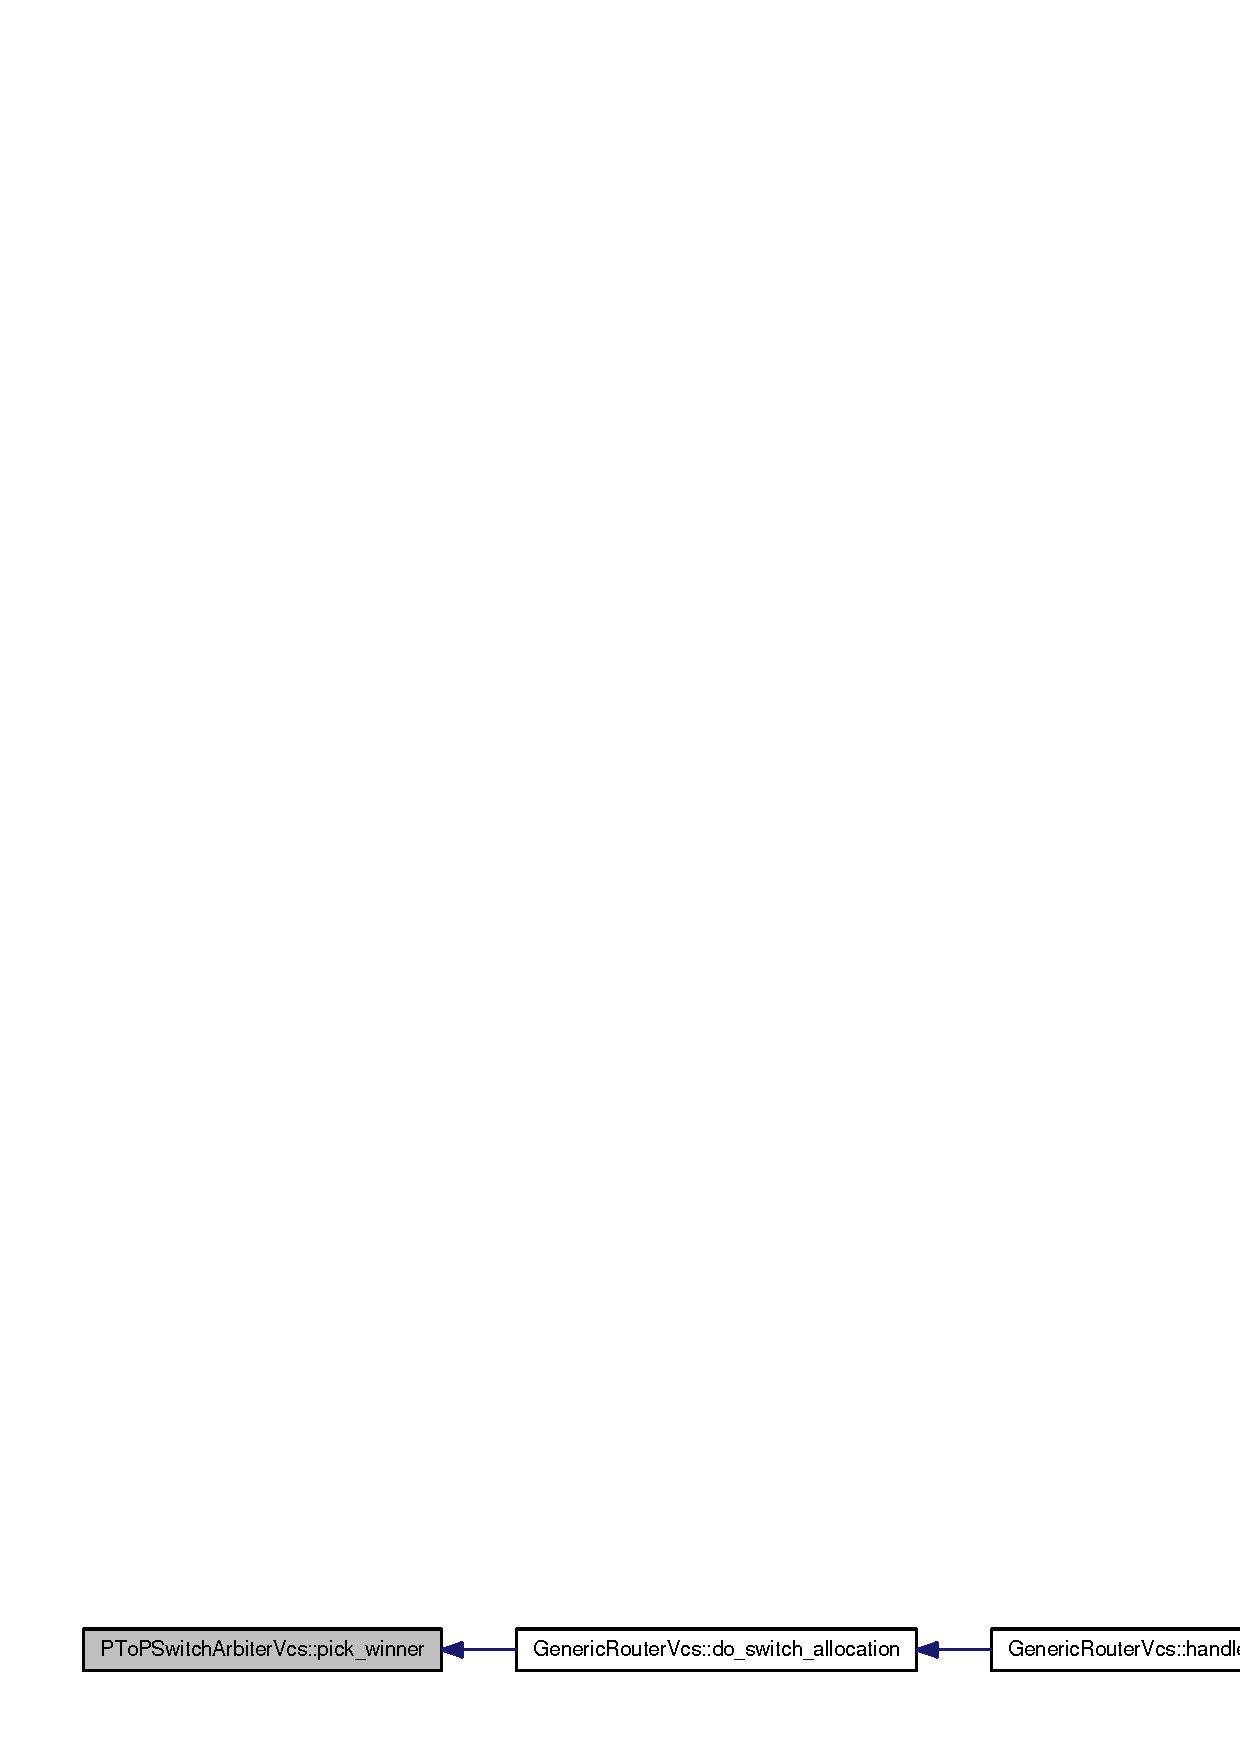
\includegraphics[width=420pt]{classPToPSwitchArbiterVcs_39274b4ccaad44c9217f150a30bba0e7_icgraph}
\end{center}
\end{figure}
\index{PToPSwitchArbiterVcs@{PToPSwitchArbiterVcs}!request@{request}}
\index{request@{request}!PToPSwitchArbiterVcs@{PToPSwitchArbiterVcs}}
\subsubsection[{request}]{\setlength{\rightskip}{0pt plus 5cm}void PToPSwitchArbiterVcs::request ({\bf uint} {\em oport}, \/  {\bf uint} {\em inport}, \/  {\bf message\_\-class} {\em m})}\label{classPToPSwitchArbiterVcs_1dfd11303e490a337f7c6eec659cedfc}


\index{PToPSwitchArbiterVcs@{PToPSwitchArbiterVcs}!request@{request}}
\index{request@{request}!PToPSwitchArbiterVcs@{PToPSwitchArbiterVcs}}
\subsubsection[{request}]{\setlength{\rightskip}{0pt plus 5cm}void PToPSwitchArbiterVcs::request ({\bf uint} {\em p}, \/  {\bf uint} {\em op}, \/  {\bf uint} {\em inp}, \/  {\bf uint} {\em iv})}\label{classPToPSwitchArbiterVcs_abe8b9b7e2197d9b9b71648c80fb5489}




Definition at line 74 of file ptopSwaVcs.cc.

References Simulator::Now(), requested, requesting\_\-inputs, and vcs.

Referenced by GenericRouterVcs::do\_\-switch\_\-traversal(), and GenericRouterVcs::handle\_\-tick\_\-event().

Here is the caller graph for this function:\nopagebreak
\begin{figure}[H]
\begin{center}
\leavevmode
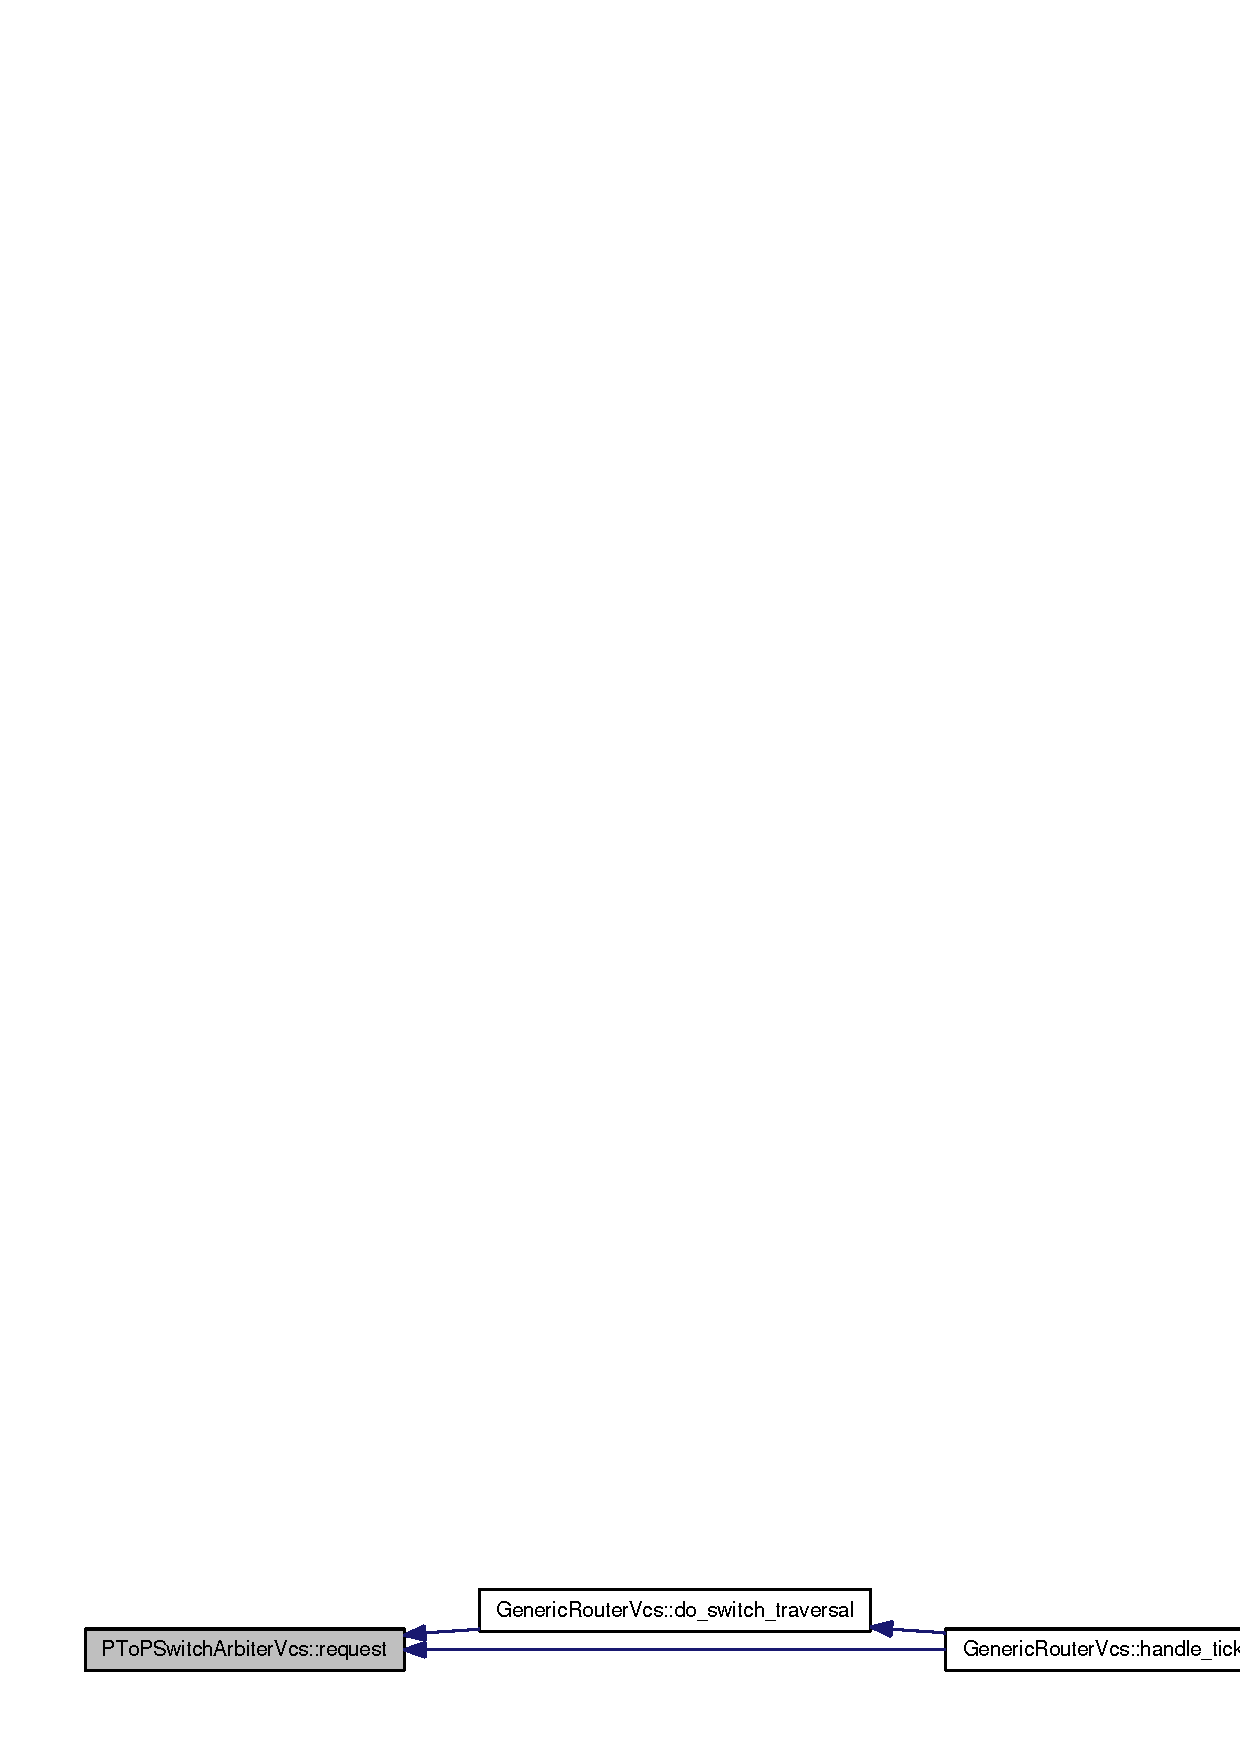
\includegraphics[width=420pt]{classPToPSwitchArbiterVcs_abe8b9b7e2197d9b9b71648c80fb5489_icgraph}
\end{center}
\end{figure}
\index{PToPSwitchArbiterVcs@{PToPSwitchArbiterVcs}!resize@{resize}}
\index{resize@{resize}!PToPSwitchArbiterVcs@{PToPSwitchArbiterVcs}}
\subsubsection[{resize}]{\setlength{\rightskip}{0pt plus 5cm}void PToPSwitchArbiterVcs::resize ({\bf uint} {\em p}, \/  {\bf uint} {\em v})}\label{classPToPSwitchArbiterVcs_f5c5a064d2a62465cd28a5e3e7e61ea0}




Definition at line 34 of file ptopSwaVcs.cc.

References last\_\-port\_\-winner, last\_\-winner, ports, priority\_\-reqs, requested, requesting\_\-inputs, and vcs.

Referenced by GenericRouterVcs::init().

Here is the caller graph for this function:\nopagebreak
\begin{figure}[H]
\begin{center}
\leavevmode
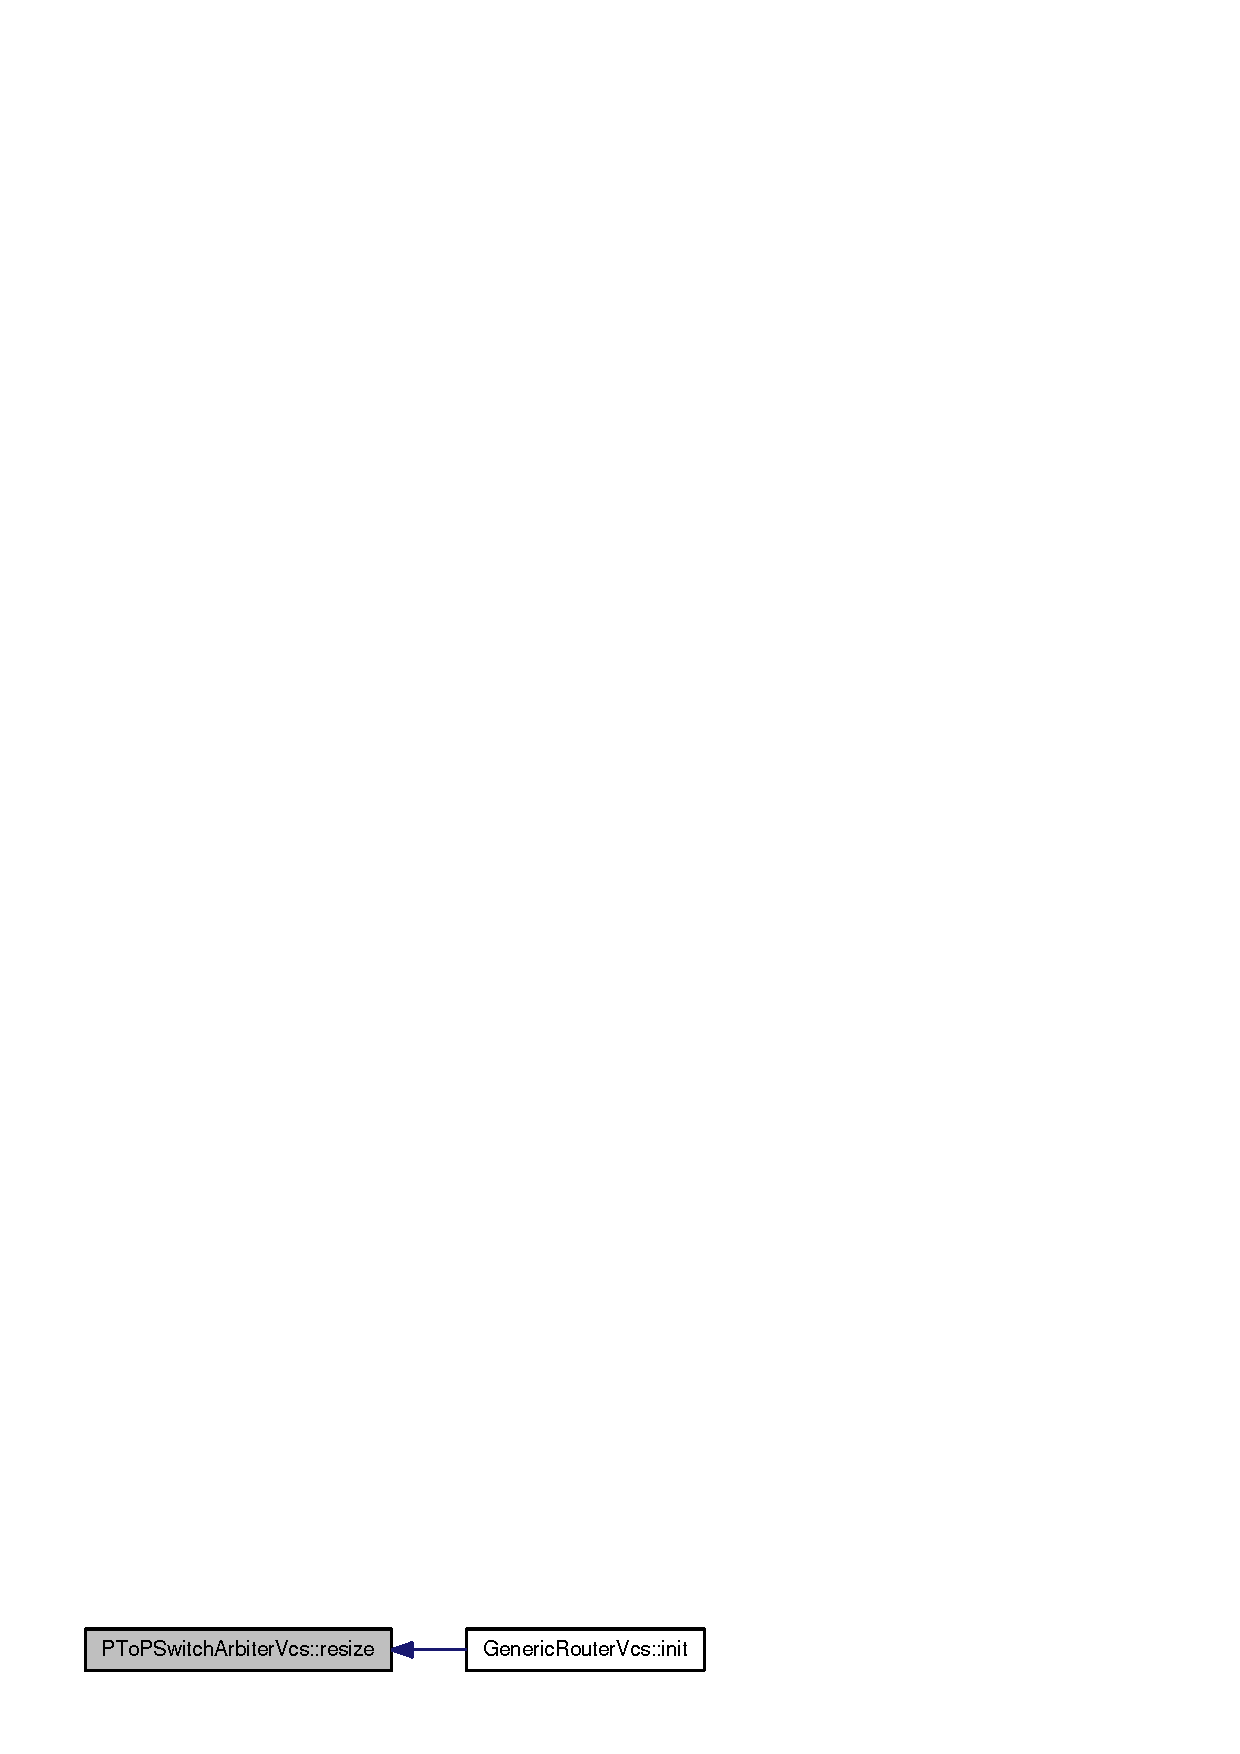
\includegraphics[width=171pt]{classPToPSwitchArbiterVcs_f5c5a064d2a62465cd28a5e3e7e61ea0_icgraph}
\end{center}
\end{figure}
\index{PToPSwitchArbiterVcs@{PToPSwitchArbiterVcs}!toString@{toString}}
\index{toString@{toString}!PToPSwitchArbiterVcs@{PToPSwitchArbiterVcs}}
\subsubsection[{toString}]{\setlength{\rightskip}{0pt plus 5cm}string PToPSwitchArbiterVcs::toString () const}\label{classPToPSwitchArbiterVcs_94cdb12d291667d5606a117417c8e339}




Definition at line 157 of file ptopSwaVcs.cc.

References requested.

Referenced by GenericRouterVcs::toString().

Here is the caller graph for this function:\nopagebreak
\begin{figure}[H]
\begin{center}
\leavevmode
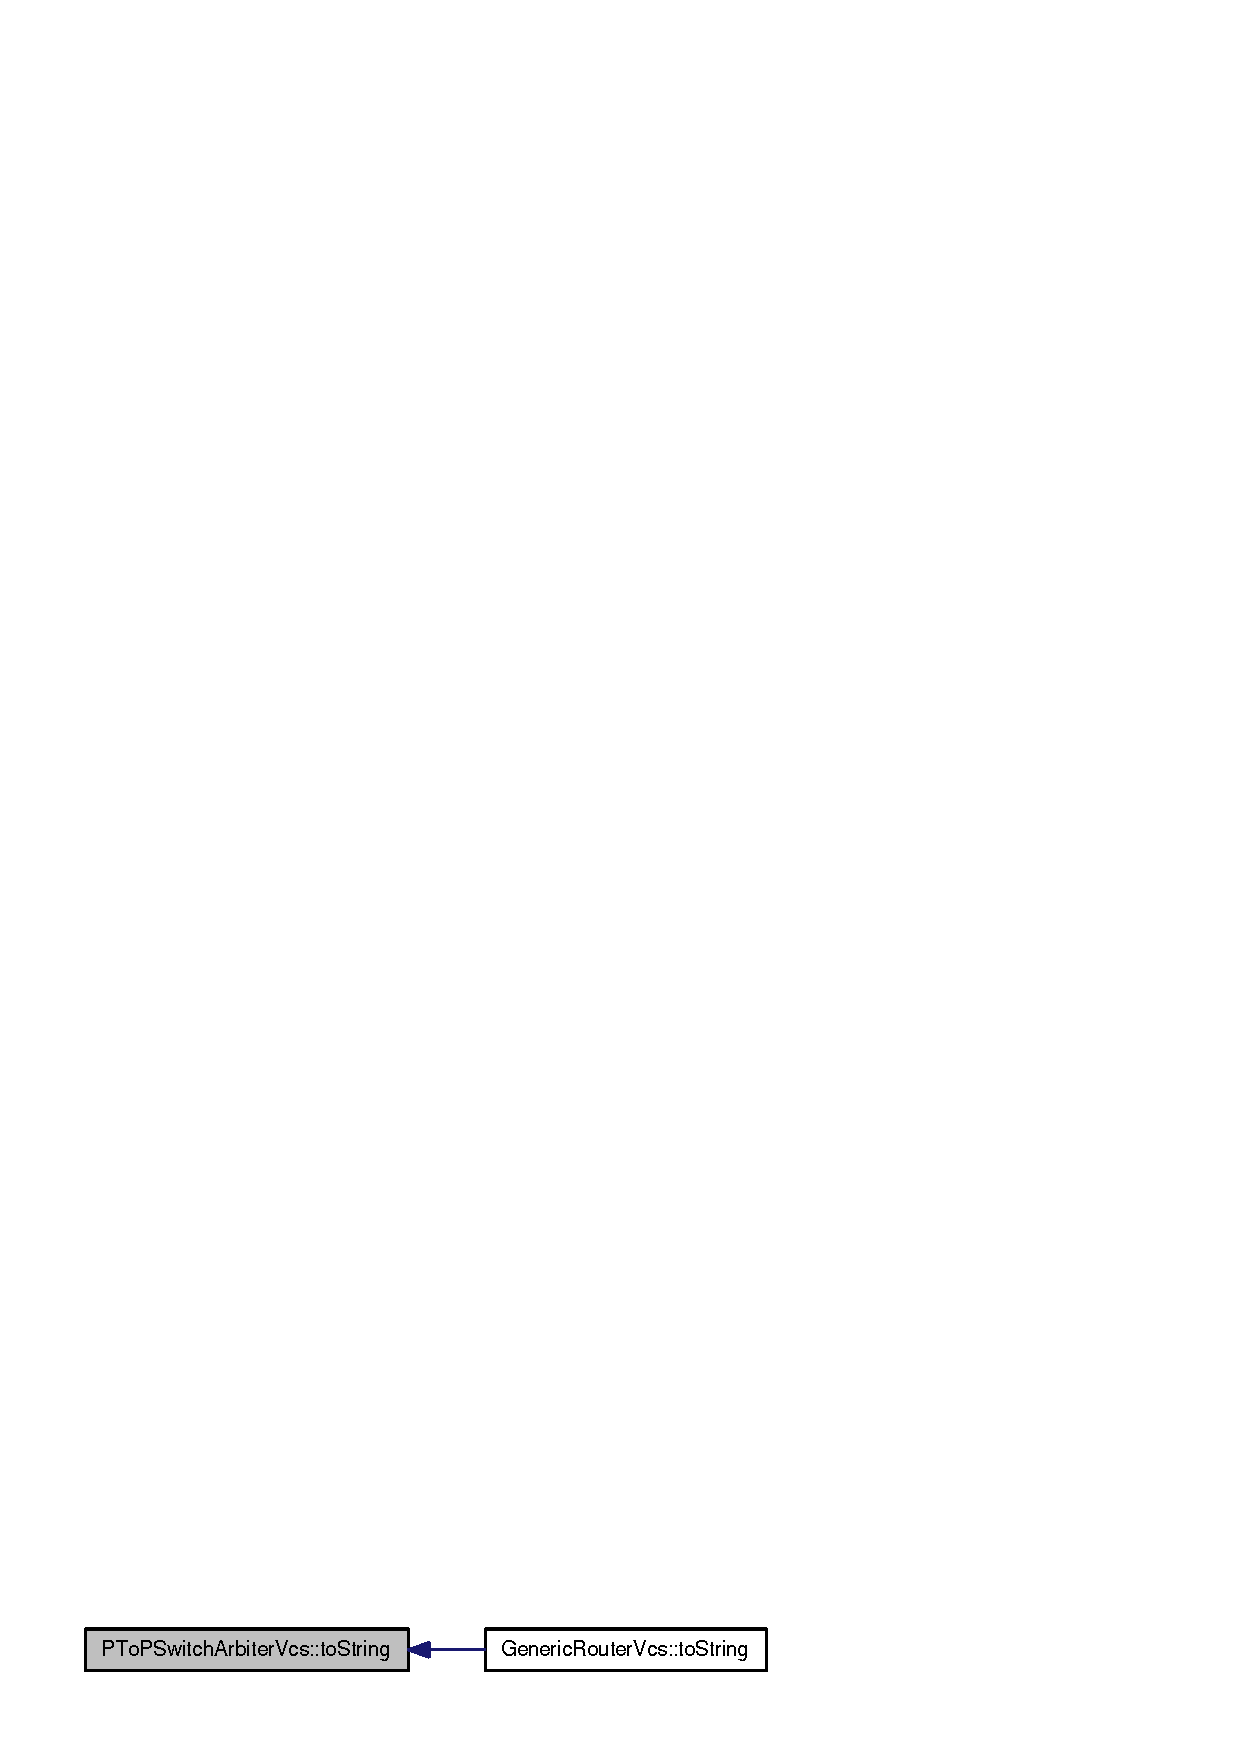
\includegraphics[width=186pt]{classPToPSwitchArbiterVcs_94cdb12d291667d5606a117417c8e339_icgraph}
\end{center}
\end{figure}


\subsection{Member Data Documentation}
\index{PToPSwitchArbiterVcs@{PToPSwitchArbiterVcs}!address@{address}}
\index{address@{address}!PToPSwitchArbiterVcs@{PToPSwitchArbiterVcs}}
\subsubsection[{address}]{\setlength{\rightskip}{0pt plus 5cm}{\bf uint} {\bf PToPSwitchArbiterVcs::address}}\label{classPToPSwitchArbiterVcs_a9a747e4c117b88e7871fc41be02d734}




Definition at line 46 of file ptopSwaVcs.h.

Referenced by GenericRouterVcs::init().\index{PToPSwitchArbiterVcs@{PToPSwitchArbiterVcs}!last\_\-port\_\-winner@{last\_\-port\_\-winner}}
\index{last\_\-port\_\-winner@{last\_\-port\_\-winner}!PToPSwitchArbiterVcs@{PToPSwitchArbiterVcs}}
\subsubsection[{last\_\-port\_\-winner}]{\setlength{\rightskip}{0pt plus 5cm}vector$<$ {\bf uint}$>$ {\bf PToPSwitchArbiterVcs::last\_\-port\_\-winner}\hspace{0.3cm}{\tt  [private]}}\label{classPToPSwitchArbiterVcs_d8a65d4ecb52149d431ee6c29e776941}




Definition at line 59 of file ptopSwaVcs.h.

Referenced by do\_\-round\_\-robin\_\-arbitration(), and resize().\index{PToPSwitchArbiterVcs@{PToPSwitchArbiterVcs}!last\_\-winner@{last\_\-winner}}
\index{last\_\-winner@{last\_\-winner}!PToPSwitchArbiterVcs@{PToPSwitchArbiterVcs}}
\subsubsection[{last\_\-winner}]{\setlength{\rightskip}{0pt plus 5cm}vector$<$ {\bf SA\_\-unit} $>$ {\bf PToPSwitchArbiterVcs::last\_\-winner}\hspace{0.3cm}{\tt  [private]}}\label{classPToPSwitchArbiterVcs_a6b5938bab8fdff0a73c1e16efd8560f}




Definition at line 58 of file ptopSwaVcs.h.

Referenced by do\_\-round\_\-robin\_\-arbitration(), and resize().\index{PToPSwitchArbiterVcs@{PToPSwitchArbiterVcs}!name@{name}}
\index{name@{name}!PToPSwitchArbiterVcs@{PToPSwitchArbiterVcs}}
\subsubsection[{name}]{\setlength{\rightskip}{0pt plus 5cm}string {\bf PToPSwitchArbiterVcs::name}}\label{classPToPSwitchArbiterVcs_57ac7f9cfd7322643f12c550ae9b1171}




Definition at line 47 of file ptopSwaVcs.h.

Referenced by PToPSwitchArbiterVcs().\index{PToPSwitchArbiterVcs@{PToPSwitchArbiterVcs}!node\_\-ip@{node\_\-ip}}
\index{node\_\-ip@{node\_\-ip}!PToPSwitchArbiterVcs@{PToPSwitchArbiterVcs}}
\subsubsection[{node\_\-ip}]{\setlength{\rightskip}{0pt plus 5cm}{\bf uint} {\bf PToPSwitchArbiterVcs::node\_\-ip}}\label{classPToPSwitchArbiterVcs_0366e83fa194f5e5ef6ac5fe628e70fb}




Definition at line 48 of file ptopSwaVcs.h.

Referenced by GenericRouterVcs::init().\index{PToPSwitchArbiterVcs@{PToPSwitchArbiterVcs}!ports@{ports}}
\index{ports@{ports}!PToPSwitchArbiterVcs@{PToPSwitchArbiterVcs}}
\subsubsection[{ports}]{\setlength{\rightskip}{0pt plus 5cm}{\bf uint} {\bf PToPSwitchArbiterVcs::ports}\hspace{0.3cm}{\tt  [private]}}\label{classPToPSwitchArbiterVcs_7b971bdd0d68a0e81e192312f51a5c4a}




Definition at line 53 of file ptopSwaVcs.h.

Referenced by do\_\-round\_\-robin\_\-arbitration(), is\_\-empty(), is\_\-requested(), and resize().\index{PToPSwitchArbiterVcs@{PToPSwitchArbiterVcs}!priority\_\-reqs@{priority\_\-reqs}}
\index{priority\_\-reqs@{priority\_\-reqs}!PToPSwitchArbiterVcs@{PToPSwitchArbiterVcs}}
\subsubsection[{priority\_\-reqs}]{\setlength{\rightskip}{0pt plus 5cm}vector$<$ vector $<$bool$>$ $>$ {\bf PToPSwitchArbiterVcs::priority\_\-reqs}\hspace{0.3cm}{\tt  [private]}}\label{classPToPSwitchArbiterVcs_ce903c8ba11cf00d738dc14c7af152c2}




Definition at line 56 of file ptopSwaVcs.h.

Referenced by resize().\index{PToPSwitchArbiterVcs@{PToPSwitchArbiterVcs}!requested@{requested}}
\index{requested@{requested}!PToPSwitchArbiterVcs@{PToPSwitchArbiterVcs}}
\subsubsection[{requested}]{\setlength{\rightskip}{0pt plus 5cm}vector$<$ vector $<$bool$>$ $>$ {\bf PToPSwitchArbiterVcs::requested}\hspace{0.3cm}{\tt  [private]}}\label{classPToPSwitchArbiterVcs_3b8835d4168422f28451087b513dc1d8}




Definition at line 55 of file ptopSwaVcs.h.

Referenced by clear\_\-requestor(), do\_\-round\_\-robin\_\-arbitration(), is\_\-empty(), is\_\-requested(), request(), resize(), and toString().\index{PToPSwitchArbiterVcs@{PToPSwitchArbiterVcs}!requesting\_\-inputs@{requesting\_\-inputs}}
\index{requesting\_\-inputs@{requesting\_\-inputs}!PToPSwitchArbiterVcs@{PToPSwitchArbiterVcs}}
\subsubsection[{requesting\_\-inputs}]{\setlength{\rightskip}{0pt plus 5cm}vector$<$ vector$<${\bf SA\_\-unit}$>$ $>$ {\bf PToPSwitchArbiterVcs::requesting\_\-inputs}\hspace{0.3cm}{\tt  [private]}}\label{classPToPSwitchArbiterVcs_454d0d84471682e1563ae6b1b4c4da5d}




Definition at line 57 of file ptopSwaVcs.h.

Referenced by do\_\-round\_\-robin\_\-arbitration(), request(), and resize().\index{PToPSwitchArbiterVcs@{PToPSwitchArbiterVcs}!vcs@{vcs}}
\index{vcs@{vcs}!PToPSwitchArbiterVcs@{PToPSwitchArbiterVcs}}
\subsubsection[{vcs}]{\setlength{\rightskip}{0pt plus 5cm}{\bf uint} {\bf PToPSwitchArbiterVcs::vcs}\hspace{0.3cm}{\tt  [private]}}\label{classPToPSwitchArbiterVcs_119836b981999b12f4cc2d9c8b9cdcbc}




Definition at line 54 of file ptopSwaVcs.h.

Referenced by clear\_\-requestor(), do\_\-round\_\-robin\_\-arbitration(), is\_\-empty(), is\_\-requested(), request(), and resize().

The documentation for this class was generated from the following files:\begin{CompactItemize}
\item 
{\bf ptopSwaVcs.h}\item 
{\bf ptopSwaVcs.cc}\end{CompactItemize}
